\begin{figure}
    \centering
    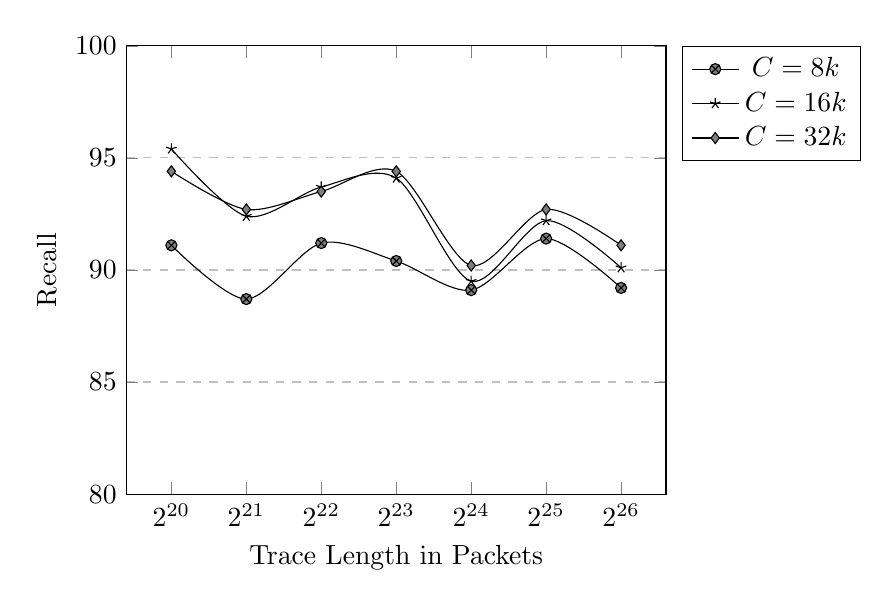
\begin{tikzpicture}
        \begin{axis}[
        xlabel={Trace Length in Packets},
        ylabel={Recall},
        xtick=data,
        xticklabels={$2^{20}$, $2^{21}$, $2^{22}$, $2^{23}$, $2^{24}$, $2^{25}$, $2^{26}$},
        ytick={0,5,10,15,20,25,30,35,40,45,50,55,60,65,70,75,80,85,90,95,100},
        % legend pos=south east,
        % legend columns=2,
        ymajorgrids=true,
        ymax=100,
        ymin=80,
        grid style=dashed,
        legend style ={ at={(1.03,1)}, 
        anchor=north west, draw=black, 
        fill=white,align=left},
        cycle list name=black white,
        smooth
        ]
            \addplot
            coordinates {
                (1,91.1)(2,88.7)(3,91.2)(4,90.4)(5,89.1)(6,91.4)(7,89.2)
            };
            \addlegendentry{$C=8k$};
            \addplot
            coordinates {
                (1,95.4)(2,92.4)(3,93.7)(4,94.1)(5,89.5)(6,92.2)(7,90.1)
            };
            \addlegendentry{$C=16k$};
            \pgfplotsset{cycle list shift=2}
            \addplot
            coordinates {
                (1,94.4)(2,92.7)(3,93.5)(4,94.4)(5,90.2)(6,92.7)(7,91.1)
            };
            \addlegendentry{$C=32k$};
        \end{axis}
    \end{tikzpicture}
    \caption[Recall of ~\ref{algo:sa} Algorithm as function of the trace length]{The recall of~\ref{algo:sa} Algorithm for various length of trace on CAIDA'18.}
    \label{fig:trace_length}
\end{figure}